\documentclass[
    fontsize=12pt,          % default font size 12pt
    paper=a4,               % DIN A4 page format
    numbers=noenddot,       % remove dots behind chapter numbers (e.g. 1.5 not 1.5.)
    listof=totoc,           % add list of figures, tables, etc. to ToC
    listof=entryprefix,     % add entry name to figures, tables, etc.
    listof=nochaptergap,    % no chapter gap for figures, tables, etc.
    bibliography=totoc,     % add bibliography to ToC but without a chapter number
    parskip=half,           % half line spacing between paragraphs
    openany                 % chapters can start on any page
]{scrbook}

\include{../../for_latex/preamble}

\usepackage{tikz}
\usetikzlibrary{mindmap}

\begin{document}

    \begin{titlepage}
        \pagestyle{empty}

        % HFU Logo
        \begin{flushright}
            \begin{figure}[ht]
                \flushright
                
\includegraphics[height=2cm]{../../for_latex/hfu}
            \end{figure}
        \end{flushright}

        \begin{center}
            \vspace{3cm}

            {\fontsize{22}{22} \selectfont \textbf{Blatt 1}}\\[5mm]
            {\fontsize{18}{18} \selectfont Kryptologie}

            \vspace{12cm}

            {\fontsize{14}{14} \selectfont Luis Staudt}
        \end{center}
    \end{titlepage}

% ############################################################################
% CONTENT STARTS HERE
% ############################################################################


\chapter*{Analyse eines LFSR-PRNG}


\section*{Aufgabenstellung}

Es soll ein Linear Feedback Shift Register (LFSR) vom Fibonacci-Typ der Länge 16 analysiert werden.
Das Generatorpolynom lautet:
\[
    g(x) = x^{16} + x^{10} + x^{6} + x^{5} + 1
\]
Der Initialwert (als Bitfolge) ist:
\[
    (1,\; 0,\; 0,\; 1,\; 0,\; 0,\; 0,\; 0,\; 0,\; 0,\; 1,\; 1,\; 1,\; 1,\; 1,\; 1)
\]
Es werden 20000 Bits erzeugt und anschließend mit dem Monobit-Test, dem Poker-Test und dem Run-Test auf statistische Zufälligkeit geprüft.
Die Annahmebereiche richten sich nach NIST FIPS140-2 und BSI AIS 31.

Die ersten und letzten 25 erzeugten Bits lauten:
\begin{align*}
    \text{Erste 25 Bits:} \quad & 1\;1\;1\;1\;1\;1\;0\;0\;0\;0\;0\;0\;1\;0\;0\;1\;1\;0\;0\;1\;0\;1\;0\;0\;1 \\
    \text{Letzte 25 Bits:} \quad & 1\;0\;0\;1\;0\;0\;0\;1\;1\;0\;0\;0\;1\;0\;1\;1\;1\;0\;0\;0\;0\;0\;0\;1\;0
\end{align*}


\section*{Vorgehensweise}

Die Implementierung erfolgt in Python.
Das LFSR wird als Array der Länge 16 realisiert.
In jedem Takt wird das Ausgabebit (Position 16) entnommen und das Feedback als XOR der Positionen 16, 10, 6 und 5 berechnet.
Anschließend wird das Register nach rechts geschoben und das Feedback-Bit an Position 1 eingefügt.

\begin{lstlisting}[language=Python, caption={LFSR-Implementierung}]
lfsr = [1, 0, 0, 1, 0, 0, 0, 0, 0, 0, 1, 1, 1, 1, 1, 1]
bits = []
for i in range(20000):
    output = lfsr[15]
    bits.append(output)
    fb = (lfsr[15] + lfsr[9] + lfsr[5] + lfsr[4]) % 2
    lfsr = [fb] + lfsr[:15]
\end{lstlisting}


\section*{Monobit-Test}

Der Monobit-Test zählt die Anzahl der Einsen $X$ in der gesamten Bitsequenz.
Bei einer idealen Zufallsfolge erwartet man $X \approx 10000$.

\begin{table}[H]
    \centering
    \begin{tabular}{l c c c}
        \toprule
        \textbf{Test bestanden gemäß} & \textbf{Wert}               & \textbf{Annahmebereich} & \textbf{Ergebnis} \\
        \midrule
        NIST FIPS140-2                & \multirow{2}{*}{$X = 9972$} & $(9725;\; 10275)$       & bestanden         \\
        BSI AIS 31                    &                             & $(9654;\; 10346)$       & bestanden         \\
        \bottomrule
    \end{tabular}
    \caption{Ergebnis des Monobit-Tests}
\end{table}

Der Wert $X = 9972$ liegt nahe am Erwartungswert und innerhalb beider Annahmebereiche.
Der Monobit-Test ist somit bestanden.

\section*{Poker-Test}

Beim Poker-Test werden die 20000 Bits in 5000 Nibbles (je 4 Bit) aufgeteilt.
Die Zufallsgröße $f_k$ zählt die Häufigkeit jedes Nibble-Werts $k \in \{0, \ldots, 15\}$.
Die Teststatistik berechnet sich als:
\[
    Y = \frac{16}{5000} \cdot \sum_{k=0}^{15} f_k^2 - 5000
\]

\begin{table}[H]
    \centering
    \begin{tabular}{l c c c}
        \toprule
        \textbf{Test bestanden gemäß} & \textbf{Wert}                    & \textbf{Annahmebereich} & \textbf{Ergebnis} \\
        \midrule
        NIST FIPS140-2                & \multirow{2}{*}{$Y = 14{,}7968$} & $(2{,}16;\; 46{,}17)$   & bestanden         \\
        BSI AIS 31                    &                                  & $(1{,}03;\; 57{,}4)$    & bestanden         \\
        \bottomrule
    \end{tabular}
    \caption{Ergebnis des Poker-Tests}
\end{table}

Die Häufigkeitsverteilung der Nibble-Werte ist in \cref{fig:nibble} dargestellt.

\begin{figure}[H]
    \centering
    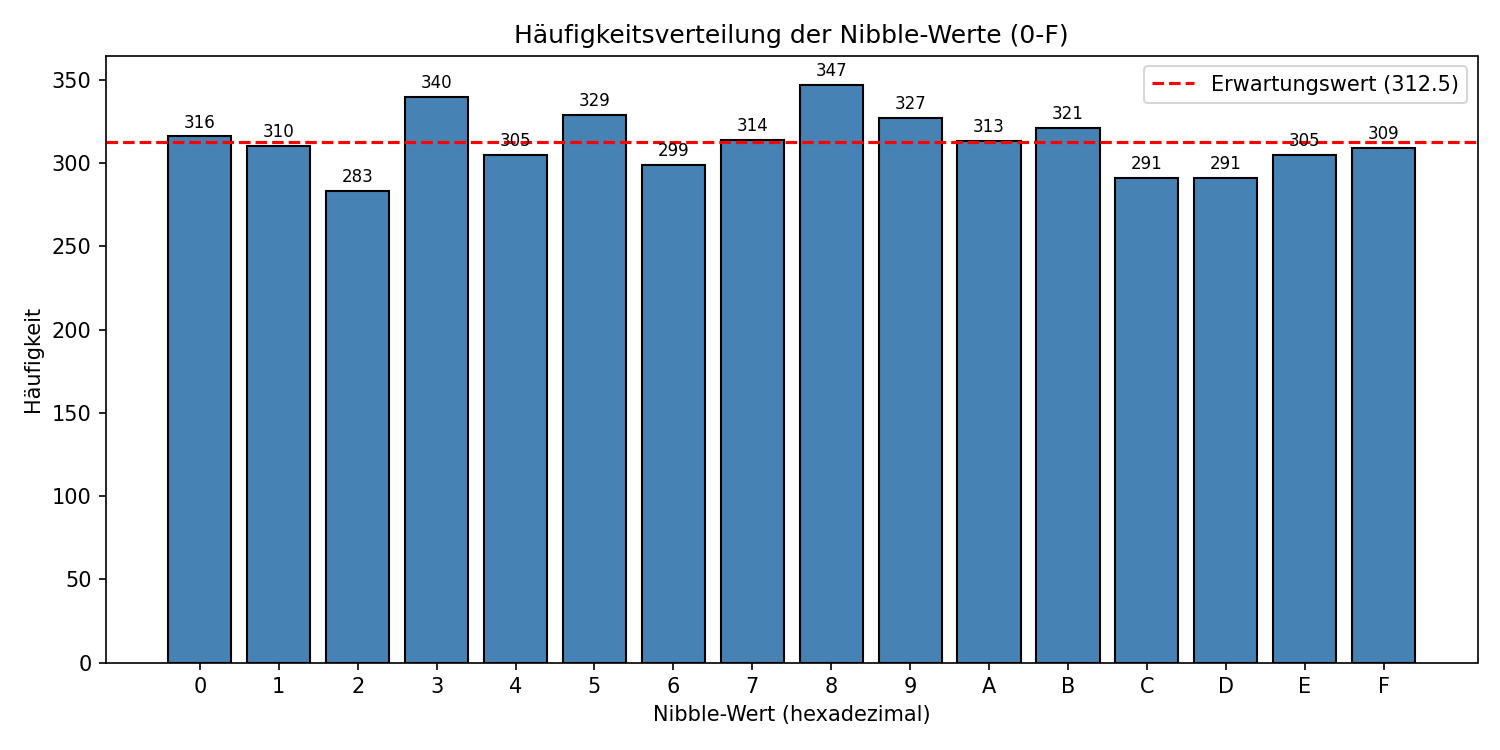
\includegraphics[width=0.9\textwidth]{nibble_histogram.png}
    \caption{Häufigkeitsverteilung der Nibble-Werte (0--F)}
    \label{fig:nibble}
\end{figure}

Die Nibble-Häufigkeiten schwanken um den Erwartungswert von $312{,}5$ und zeigen keine auffällige Abweichung.
Der Poker-Test ist bestanden.

\section*{Run-Test}

Der Run-Test untersucht die Anzahl der aufeinanderfolgenden gleichen Bits (Runs).
Es wird zwischen 0-Runs und 1-Runs unterschieden, jeweils nach Länge $k$ gruppiert.

\begin{table}[H]
    \centering
    \begin{tabular}{c r r c c c c}
        \toprule
        \textbf{Länge} & $\boldsymbol{zero_k}$ & $\boldsymbol{one_k}$ & \textbf{NIST Bereich} & \textbf{NIST} & \textbf{BSI Bereich} & \textbf{BSI} \\
        \midrule
        1              & 2476                  & 2534                 & $[2315;\; 2685]$      & best.         & $[2267;\; 2733]$     & best.        \\
        2              & 1263                  & 1207                 & $[1114;\; 1386]$      & best.         & $[1079;\; 1421]$     & best.        \\
        3              & 631                   & 621                  & $[527;\; 723]$        & best.         & $[502;\; 748]$       & best.        \\
        4              & 301                   & 329                  & $[240;\; 384]$        & best.         & $[233;\; 402]$       & best.        \\
        5              & 163                   & 134                  & $[103;\; 209]$        & best.         & $[90;\; 223]$        & best.        \\
        $\geq 6$       & 159                   & 168                  & $[103;\; 209]$        & best.         & $[90;\; 223]$        & best.        \\
        \bottomrule
    \end{tabular}
    \caption{Ergebnis des Run-Tests}
\end{table}

Die Verteilung der Runs ist in \cref{fig:runs} dargestellt.

\begin{figure}[H]
    \centering
    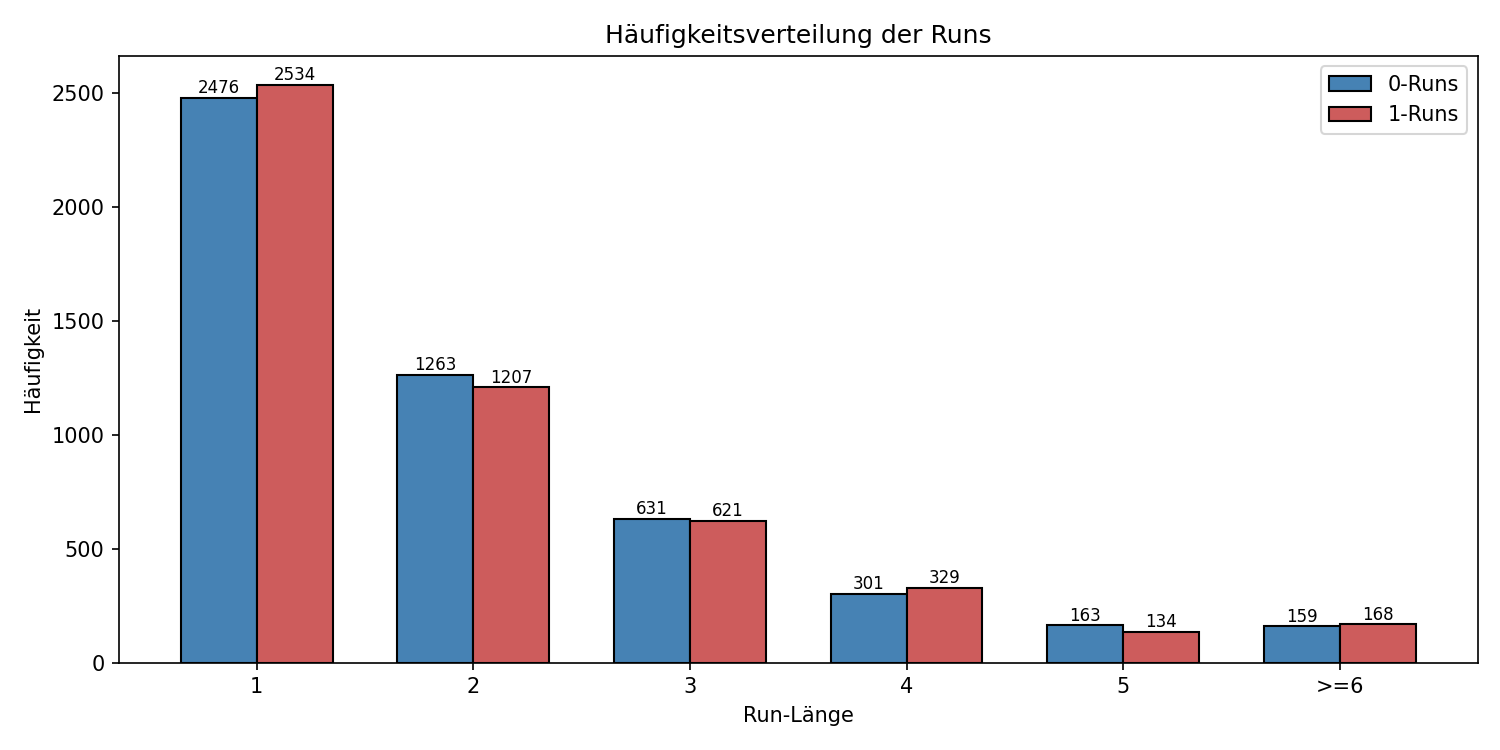
\includegraphics[width=0.9\textwidth]{run_histogram}
    \caption{Häufigkeitsverteilung der 0-Runs und 1-Runs}
    \label{fig:runs}
\end{figure}

Alle Run-Häufigkeiten liegen innerhalb der Annahmebereiche beider Standards.
Der Run-Test ist bestanden.

\section*{Long-Run-Test}

Der Long-Run-Test prüft, ob ungewöhnlich lange Runs auftreten.

\begin{table}[H]
    \centering
    \begin{tabular}{l c c c}
        \toprule
        \textbf{Test bestanden gemäß} & \textbf{Längster Run} & \textbf{Grenzwert} & \textbf{Ergebnis} \\
        \midrule
        NIST FIPS140-2                & \multirow{2}{*}{13}   & $< 34$             & bestanden         \\
        BSI AIS 31                    &                       & $< 31$             & bestanden         \\
        \bottomrule
    \end{tabular}
    \caption{Ergebnis des Long-Run-Tests}
\end{table}

Der längste aufgetretene Run hat die Länge 13 und liegt weit unter beiden Grenzwerten.


\section*{Bewertung}

Das LFSR mit dem Generatorpolynom $g(x) = x^{16} + x^{10} + x^{6} + x^{5} + 1$ besteht alle vier statistischen Zufälligkeitstests (Monobit, Poker, Run, Long-Run) sowohl nach NIST FIPS140-2 als auch nach BSI AIS 31.
Die erzeugten 20000 Bits weisen eine gleichmäßige Verteilung der Einsen und Nullen auf, die Nibble-Häufigkeiten schwanken nahe am Erwartungswert und die Run-Längen liegen in den erwarteten Bereichen.

Das Generatorpolynom erzeugt somit eine Bitfolge, die grundlegende statistische Zufälligkeitsanforderungen erfüllt.
Es ist jedoch zu beachten, dass diese Tests notwendige, aber nicht hinreichende Bedingungen für kryptographische Sicherheit sind.
Ein LFSR allein ist als kryptographischer Zufallsgenerator nicht geeignet, da die lineare Struktur durch den Berlekamp-Massey-Algorithmus leicht rekonstruiert werden kann.

% ############################################################################
% CONTENT ENDS HERE
% ############################################################################

\end{document}
